In order to evaluate the impact of having Cassandra as a datastore for \ac{sql} queries as opposed to running them on Derby, and to measure the overhead of using our transactional system we ran three different types of tests, the TPC-W benchmark, Yahoo! Cloud Serving Benchmark and scaling out process. This chapter details those tests and consequent results. 

\section{Testing Environment}
The tests were ran on HP computers with an Intel(R) Core(TM)2 CPU 6400 - 2.13 GHz processor, two Gigabytes of RAM and a SATA (7200 RPM) hard drive. The multiple machines are connected by LAN to a 1GB/s switch and run a Linux operating system, more specifically an Ubuntu Server, 2.6.31-1 kernel and an ext4 filesystem. 
All the test were run using between 2 and 8 of these machines according to the specific needs of each test. 

\section{TPC-W Benchmark}
The TPC-W benchmark specifies an e-commerce workload that simulates customers browsing, ordering and buying products from a website. The proposed solution for this benchmark is a number of servers (Web Servers, Web Caches, Image Servers and Database Server) working in concert to provide an e-commerce solution that is very similar to how an actual website performing this kind of business would operate. 

This benchmark tests various system components that are associated with such an environment, such as~\cite{tpcw}:

\begin{itemize}
	\item The simultaneous execution of multiple transaction types that span a breadth of complexity
	\item Databases consisting of many tables with a wide variety of sizes, attributes, and relationships
	\item Transaction integrity (ACID properties)
	\item Contention on data access and update
\end{itemize}

The transaction in TPC-W can be divided into two main sets, the write operations such as adding a product to the shopping cart or ordering a product and the read operations that simulate the search of products by title, author or subject or to ask for the more recent items or the ones that have sold the most. The first set of operations is called \textbf{order} and the second \textbf{browse}.

The variation of percentage of each of these sets defines three different mixes for the benchmark:

\begin{description}
	\item[Browsing] 95\% Browsing and 5\% Ordering
	\item[Shopping] 80\% Browsing and 20\% Ordering
	\item[Ordering] 50\% Browsing and 50\% Ordering
\end{description}

Most use cases where \acp{vlsd} are used perform a lot of reads and few writes (browsing through a website) therefore, we chose the Browsing mix to perform our tests.

The configurable parameters are the numbers of \acp{eb} which represent the number of clients, and the number of items in the system, all the other parameters such as the number of customer, addresses, authors or orders, are relative to these ones.

In order to compare our implementation with and without the transactional guarantees with the standard Derby Client/Server configuration, we used one machine to serve as Client, Database Server and Web Server for all three cases. For our implementation we also used one machine as a Cassandra node and another one as a Zookeeper node for the transactional system. We tested the system with 1000 items and a varying number of clients, ranging from 10 to 100 with the results for throughput and latency show in figure \ref{fig:tpm10} and \ref{fig:lat10}, respectively.

\begin{figure}[!ht]
  \begin{center}\subfigure[Throughput]{\label{fig:tpm10}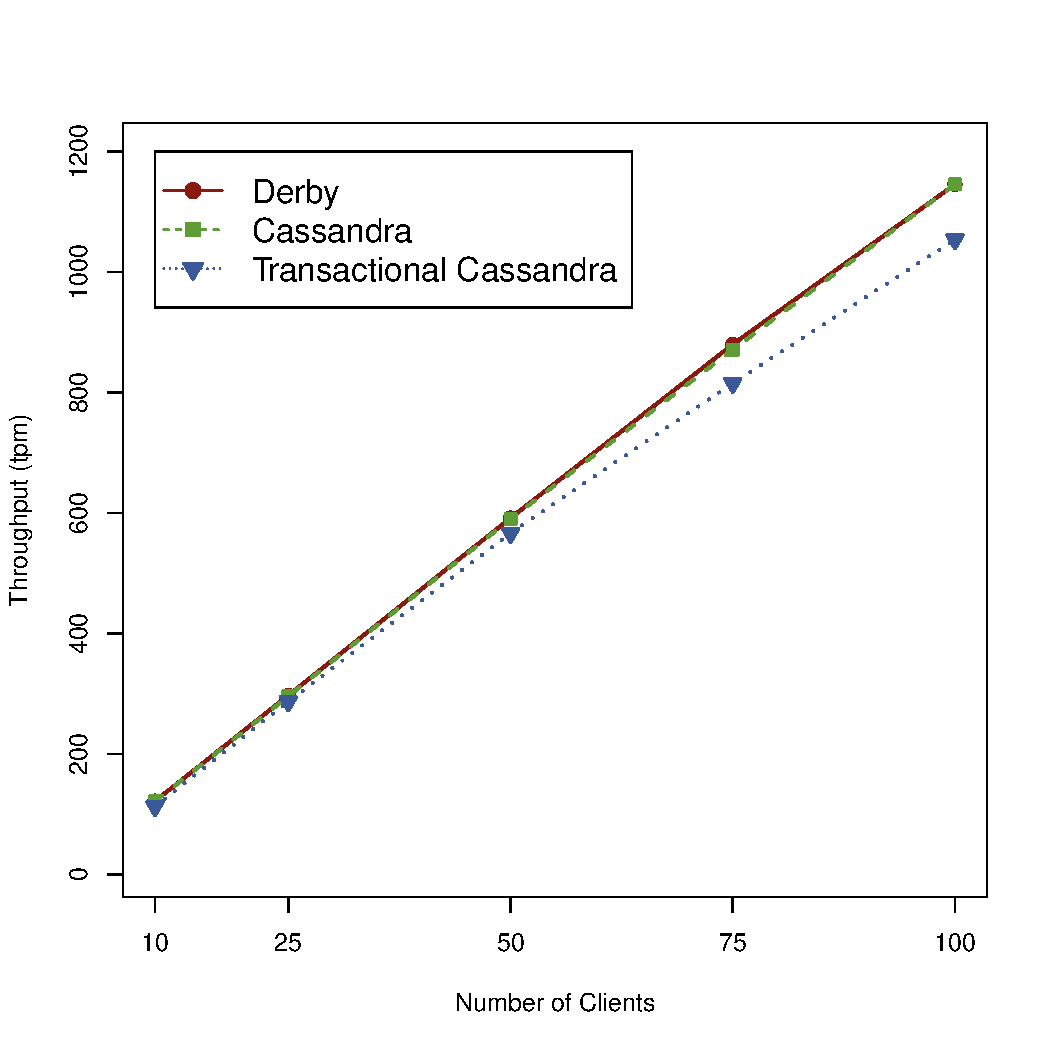
\includegraphics[width=0.7\textwidth]{images/tpcw_tpm.pdf}}\end{center}
  \begin{center}\subfigure[Latency]{\label{fig:lat10}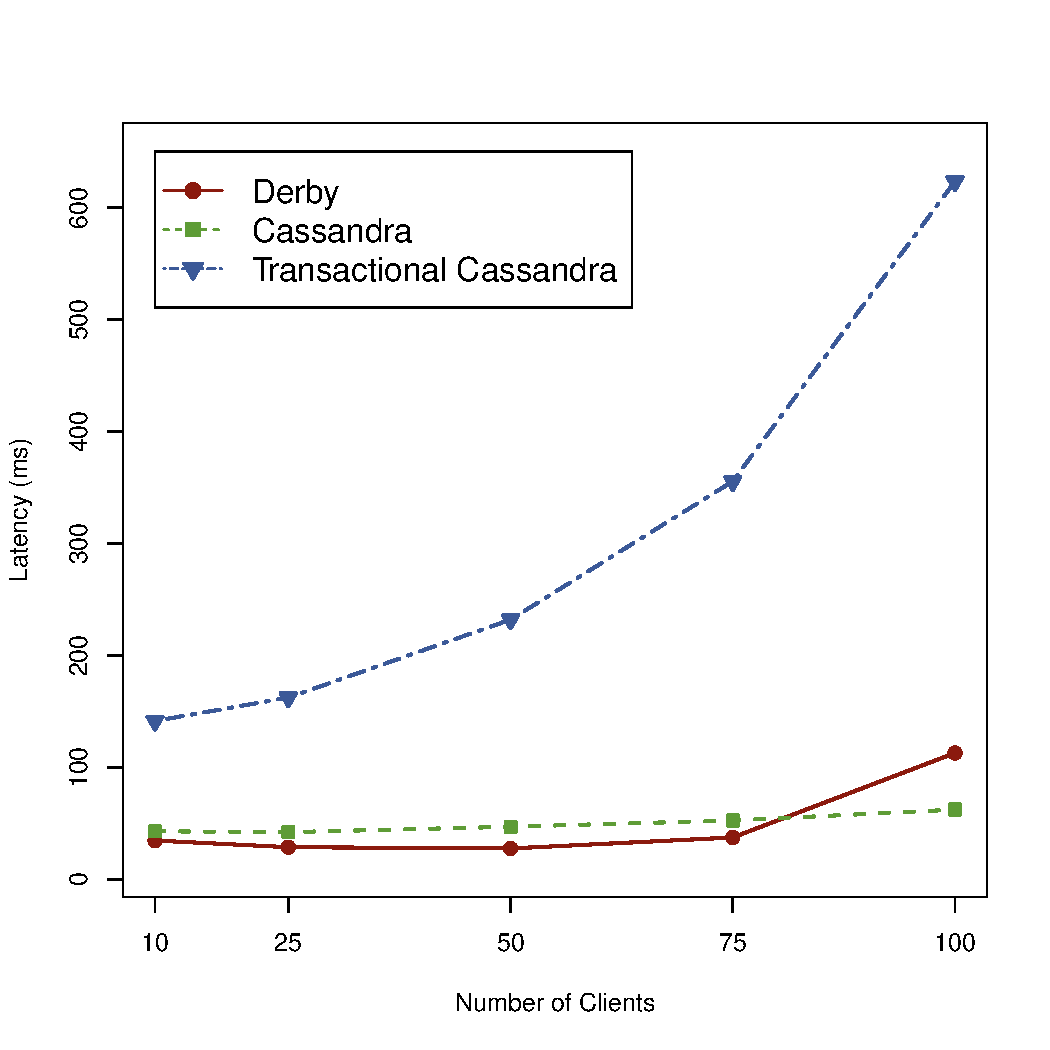
\includegraphics[width=0.7\textwidth]{images/tpcw_lat.pdf}}\end{center}
  \label{fig:tpcw10}
  \caption{Results of running TPC-W with different number of clients}
\end{figure}
 

\section{Yahoo! Cloud Serving Benchmark}

\ac{ycsb} is a framework presented by Yahoo!\footnote{\url{www.yahoo.com}} with the goal of facilitating performance comparisons of the new generation of cloud data serving systems. It focuses on \emph{serving} systems, which are systems that provide online read/write access to data such as Cassandra, as opposed to batch or analytical systems such as Hadoop~\cite{Cooper:2010:BCS:1807128.1807152}.

The workloads in the core package of \ac{ycsb} are a variation of the same application type. The application has one table of records each with \textbf{F} fields and identified by a primary key which is a string like ``user12345''. Each field is named \emph{field0}, \emph{field1}, and so on and has a random string of ASCII characters of length \textbf{L} as value. The operations against the data store are randomly chosen to be one of the following~\cite{Cooper:2010:BCS:1807128.1807152}:

\begin{description}
	\item[Insert] Insert a new record
	\item[Update] Update a record by replacing the value of multiple fields
	\item[Read] Read a record, either one randomly chosen field or all fields
	\item[Scan] Scan records in order, starting at a randomly chosen record key. The number of records to scan is randomly chosen from a configurable distribution (Uniform, Zipfian, Latest or Multinomial)
\end{description}

\ac{ycsb} also provides a tool called \ac{ycsb} Client to execute the benchmark, this tool has 5 workloads with different configurations. We introduced a new operation called multiupdate that performs updates on multiple rows, and to accommodate it we also created our own workload with 95\% reads, of which 80\% are actual read operations and 15\% are scans, and 5\% multiupdates.

For this test we used one machine running Cassandra for both the normal and transactional setting alongside with one zookeeper node for the latter. The results are shown for the scan operation are shown in figure \ref{fig:ycsb_scan}, for the read operation in figure \ref{fig:ycsb_read} and for the multiupdate in figure \ref{fig:ycsb_update}.

\begin{figure}[!ht]
  \subfigure[Scan]{\label{fig:ycsb_scan}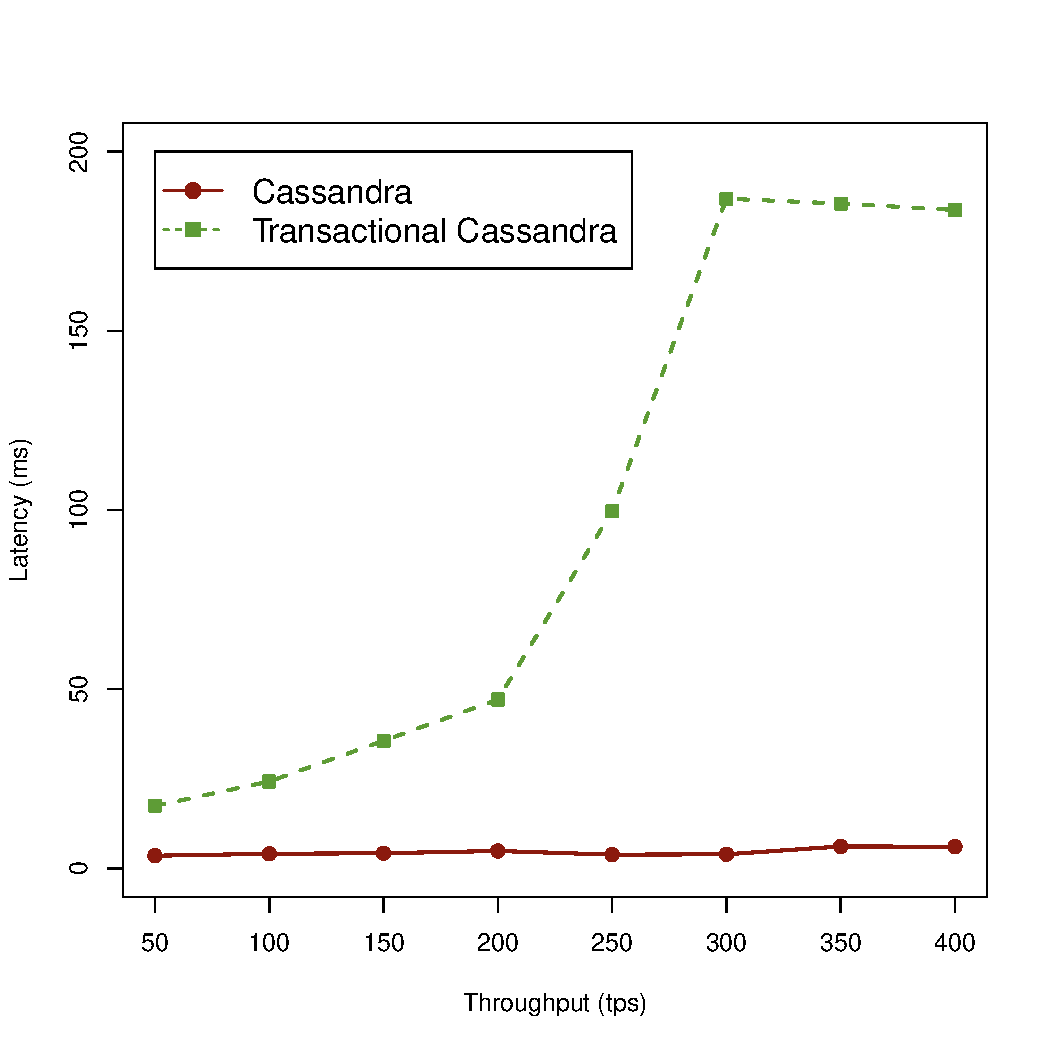
\includegraphics[width=0.5\textwidth]{images/ycsb_scan.pdf}}
  \subfigure[Read]{\label{fig:ycsb_read}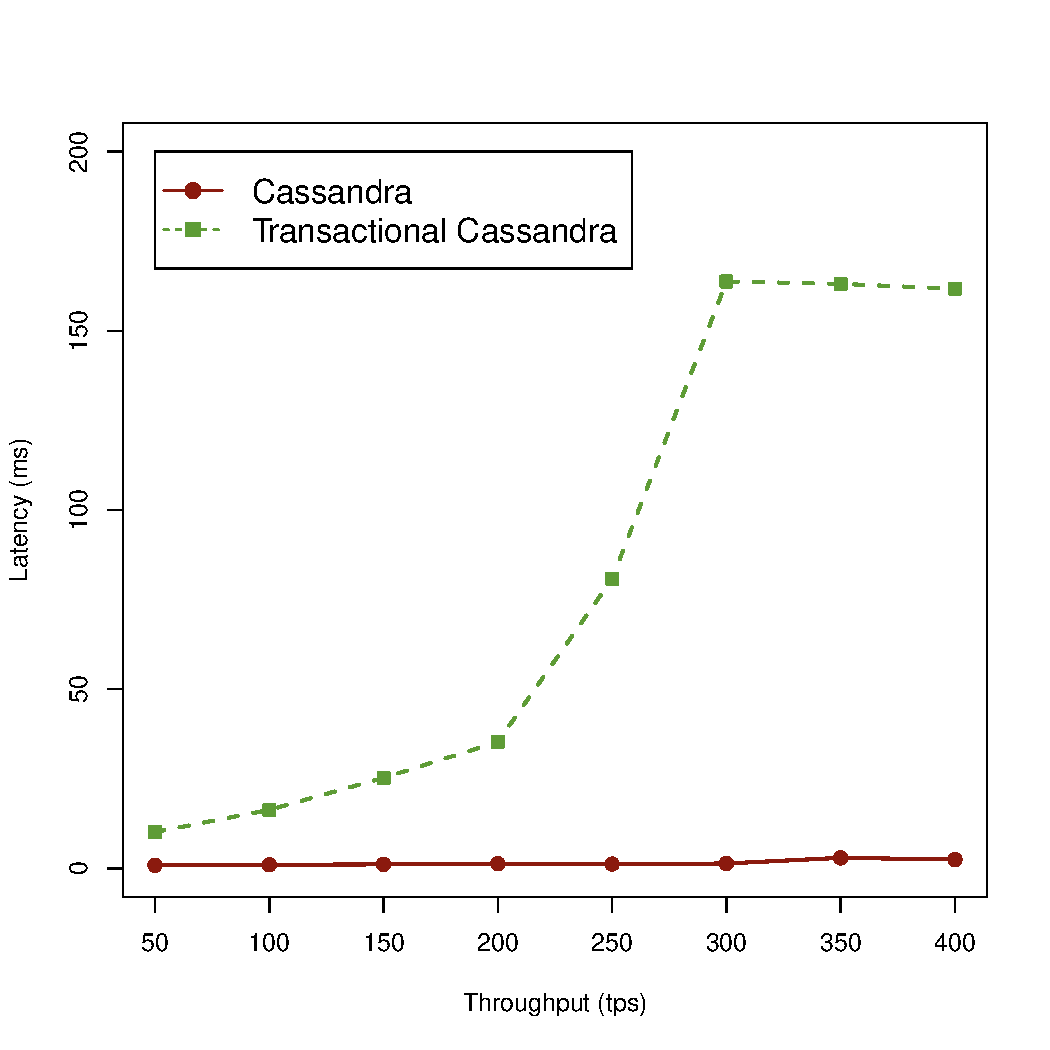
\includegraphics[width=0.5\textwidth]{images/ycsb_read.pdf}}
  \begin{center}\subfigure[Multiupdate]{\label{fig:ycsb_update}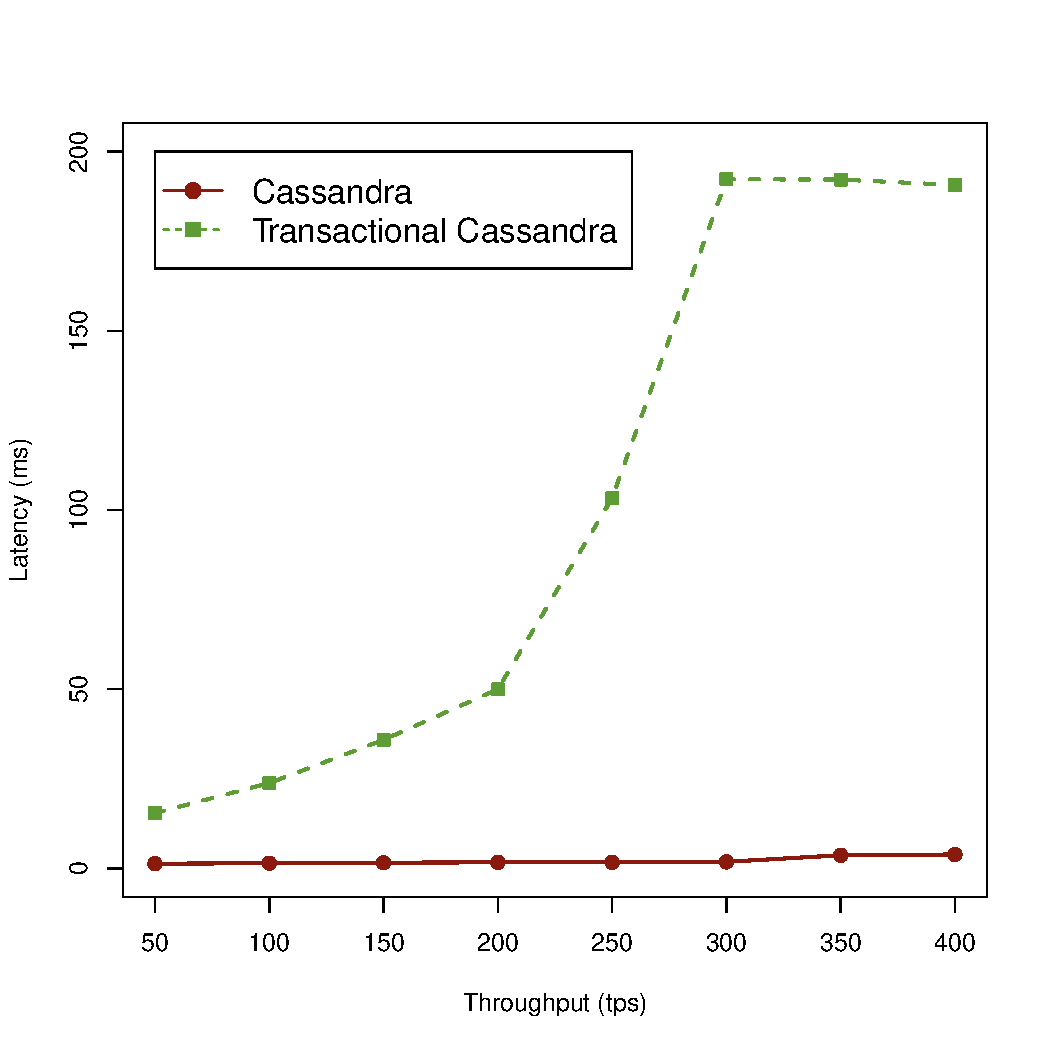
\includegraphics[width=0.5\textwidth]{images/ycsb_update.pdf}}\end{center}
  \label{fig:ycsb}
  \caption{Results of running YCSB with different expected throughput}
\end{figure}


\section{Scaling out}

So that we could better understand how the number of nodes in the cluster affected the system we tested its performance with 100 clients and 1000 items with the number of Cassandra nodes ranging from 1 to 5.  


